% -*- root: ../main.tex -*-
\chapter{Retrospettiva} \label{chap:Retrospettiva}
Questo capitolo contiene una breve retrospettiva, con i soli deliverables relativi ad ogni sprint. Per una discussione più dettagliata è possibile consultare la \href{https://github.com/ISIQuiz/ISIQuiz-Report/releases/latest/download/process.pdf}{Relazione di Processo di Sviluppo}.

\section{Svolgimento}
Gli sprint sono stati portati avanti nel seguente modo:
    \paragraph{Sprint Planning}
        Pianificazione a inizio sprint degli obiettivi, tempistiche e responsabilità nel periodo dello sprint corrente. Diviso in due parti:
        \begin{itemize}
        \item\textbf{parte 1} 
            Viene raffinato e rivisto il product backlog, viene effettuata la scelta dello sprint goal (what).
        \item\textbf{parte 2}
            Si decidono gli item e viene raffinato come implementarli (how). Effettuato con solo il team senza la figura del product owner
        \end{itemize}
    \paragraph{[Occasionale] Pair Programming} Utilizzato per risolvere problemi che causano il blocco di un componente del team per parecchio tempo su una issue.
    \paragraph{Meeting finale}
        Riflessioni e considerazioni finali sullo sprint passato. Suggerimenti per migliorare il prossimo. Diviso in tre parti: 
        \begin{itemize}
        \item\textbf{Product backlog refinement} aggiunta di dettagli e riordino del product backlog
        \item\textbf{Sprint review} è stato ispezionato l'incremento, il Minimum Viable Product o di risultati sul processo. Discernere cosa è stato fatto e cosa no
        \item\textbf{Retrospettiva} Considerazioni sul team stesso e sui miglioramenti per il prossimo sprint. 
        \end{itemize}
\section{Riepilogo Sprint}
% NOTA: le parti qui sotto sono prese dalla cartella "process", all'interno dei vari sprint, solo la "sprint review" di ognuno
\subsection{Sprint 1}
    \section{Sprint 1 Review}
%only this part is present also in the main report
Durante questo primo sprint abbiamo completato l'organizzazione di massima.
\paragraph{Deliverables} 
I deliverables per questo sprint sono stati i seguenti:
\begin{itemize}
    \item Intervista con il cliente corredata da domande
    \item Ubiquitous Language
    \item Setup Organizzazione GitHub
    \item Setup Report, con relativa repository e CI
\end{itemize}

    
\subsection{Sprint 2}
    \section{Sprint 2 Review}
%only this part is present also in the main report
Durante questo sprint abbiamo realizzato l'analisi dei requisiti del sistema e ideata l'architettura generale del sistema, dalla quale sono sorti alcuni dubbi che sono stati poi discussi e chiariti con l'esperto del dominio. Sono state realizzare due versioni dei mockup dell'applicazione, le quali hanno ricevuto entrambe giudizi positivi, ma andranno successivamente unite e raffinate per soddisfare al meglio i requisiti del committente.
\paragraph{Deliverables} 
I deliverables per questo sprint sono stati i seguenti:
\begin{itemize}
    \item Mockup
    \item Diagramma dei casi d'uso
    \item Diagramma delle classi
\end{itemize}

    
\subsection{Sprint 3}
    \section{Sprint 3 Review}
%only this part is present also in the main report
Abbiamo studiato/implementato...
\paragraph{Deliverables} 
obiettivi raggiunti
\begin{itemize}
    \item uno
    \item due
    \item tre
\end{itemize}


\subsection{Sprint 4}
    %only this part is present also in the main report.
Durante questo sprint è stata implementata completamente la visualizzazione della pagina iniziale, è stata implementata la risposta di un quiz ed è stato effettuato il setup della CI.
\paragraph{Deliverables} 
I deliverables per questo sprint sono stati i seguenti:
\begin{itemize}
    \item Visualizzazione della pagina iniziale
    \item Implementata risposta di un quiz
    \item Setup della CI 
\end{itemize}

    
\subsection{Sprint 5}
    %only this part is present also in the main report.
Durante questo sprint abbiamo sviluppato la possibilità di avviare una partita tramite utilizzando il menu principale, inoltre è stata implementata la visualizzazione delle domande e delle rispettive risposte.
\paragraph{Deliverables} 
I deliverables per questo sprint sono stati i seguenti:
\begin{itemize}
    \item Avvio di una partita;
    \item Navigazione del menu principale;
    \item Visualizzazione domande e risposte.
\end{itemize}

    
\subsection{Sprint 6}
    %only this part is present also in the main report.
Durante questo sprint sono stati implementati i meccanismi di selezione risposta e feedback su di essa. Inoltre, sono ora visibili e selezionabili i corsi disponibili prima di iniziare una partita e le domande relative ad esse sono estratte dal pool generale di quiz. Per ogni domanda inoltre, per variare l'esperienza, sono anche estratte a sorte varie possibili risposte. La sessione di ogni utente è ora salvata. Infine, è stato corretto il setup della CI.
\paragraph{Deliverables} 
I deliverables per questo sprint sono stati i seguenti:
\begin{itemize}
    \item Selezionare le risposte e ottenere dei feedback
    \item Selezione dei corsi pre-partita
    \item Visualizzazione delle opzioni di aggiunta domande
    \item Test automatici nella CI GitHub
\end{itemize}


\subsection{Sprint 7}
    %only this part is present also in the main report.
Durante questo sprint è stata implementata completamente la visualizzazione della pagina iniziale, è stata implementata la risposta di un quiz ed è stato effettuato il setup della CI.
\paragraph{Deliverables} 
I deliverables per questo sprint sono stati i seguenti:
\begin{itemize}
    \item Visualizzazione della pagina iniziale
    \item Implementata risposta di un quiz
    \item Setup della CI 
\end{itemize}

    
\subsection{Sprint 8}
    %only this part is present also in the main report.
In questo sprint non sono stati completati tutti i goal a causa dei problemi che sono sorti principalmente durante l'aggiunta dell'interfaccia grafica basata su ScalaFX. Questo ha portato a diverse problematiche di compatibilità con la parte di interfaccia grafica da linea di comando precedentemente implementata.
\paragraph{Deliverables} 
I deliverables per questo sprint sono stati i seguenti:
\begin{itemize}
    \item Create schermate dell'applicazione in FXML
    \item Aggiunta navigazione tra le pagine tramite interfaccia grafica
\end{itemize}
        
\subsection{Sprint 9}
    %only this part is also present in the main report.
In questo Sprint l'obiettivo è stato quello di finire più task possibili per dedicare la prossima iterazione ai soli refinement. La mole di lavoro svolto è stata ampia, anche grazie alla capitalizzazione del buon design, ma alcuni task sono stati rimandati successivamente.
Parte del tempo è stato dedicato alla risoluzione dei bug emersi e agli eventuali enhancements, sia grafici che della logica applicativa. Inoltre, buona parte dell'interfaccia grafica è stata implementata.
\paragraph{Deliverables} 
I deliverables per questo sprint sono stati i seguenti:
\begin{itemize}
    \item Aggiunta esportazione quiz
    \item Modifica di un corso
    \item Modifica di un quiz
    \item Visualizzazione delle statistiche
    \item Corretta visualizzazione grafica della pagina di gioco
\end{itemize}

\subsection{Sprint 10}
    %only this part is also present in the main report.
In quest'ultimo sprint ci si è focalizzati sul completamento dell'intera applicazione e sul concludere i task lasciati in precedenza. Inoltre sono stati corretti alcuni bug emersi dall'uso dell'applicazione. Ulteriori funzionalità opzionali e enhancements sono state aggiunti per completare l'applicativo e il progetto in generale.
\paragraph{Deliverables} 
I deliverables finali sono stati i seguenti:
\begin{itemize}
    \item Completata la visualizzazione delle statistiche personali
    \item Selezione della modalità di gioco
    \item Importare domande
    \item Revisione dei quiz a partita giocata
    \item Completata l'interfaccia grafica
    \item Guida utente
\end{itemize}

\section{Diagramma di Gantt}
    Durante i vari sprint è stato aggiornato anche il diagramma di Gantt creato inizialmente su Jira, come visibile nel paragrafo \ref{par:gantt}. Di seguito, nella Figura \ref{fig:jira-final} si può vedere la versione finale del diagramma con le user story.
        \begin{figure}[H]
            \centering
            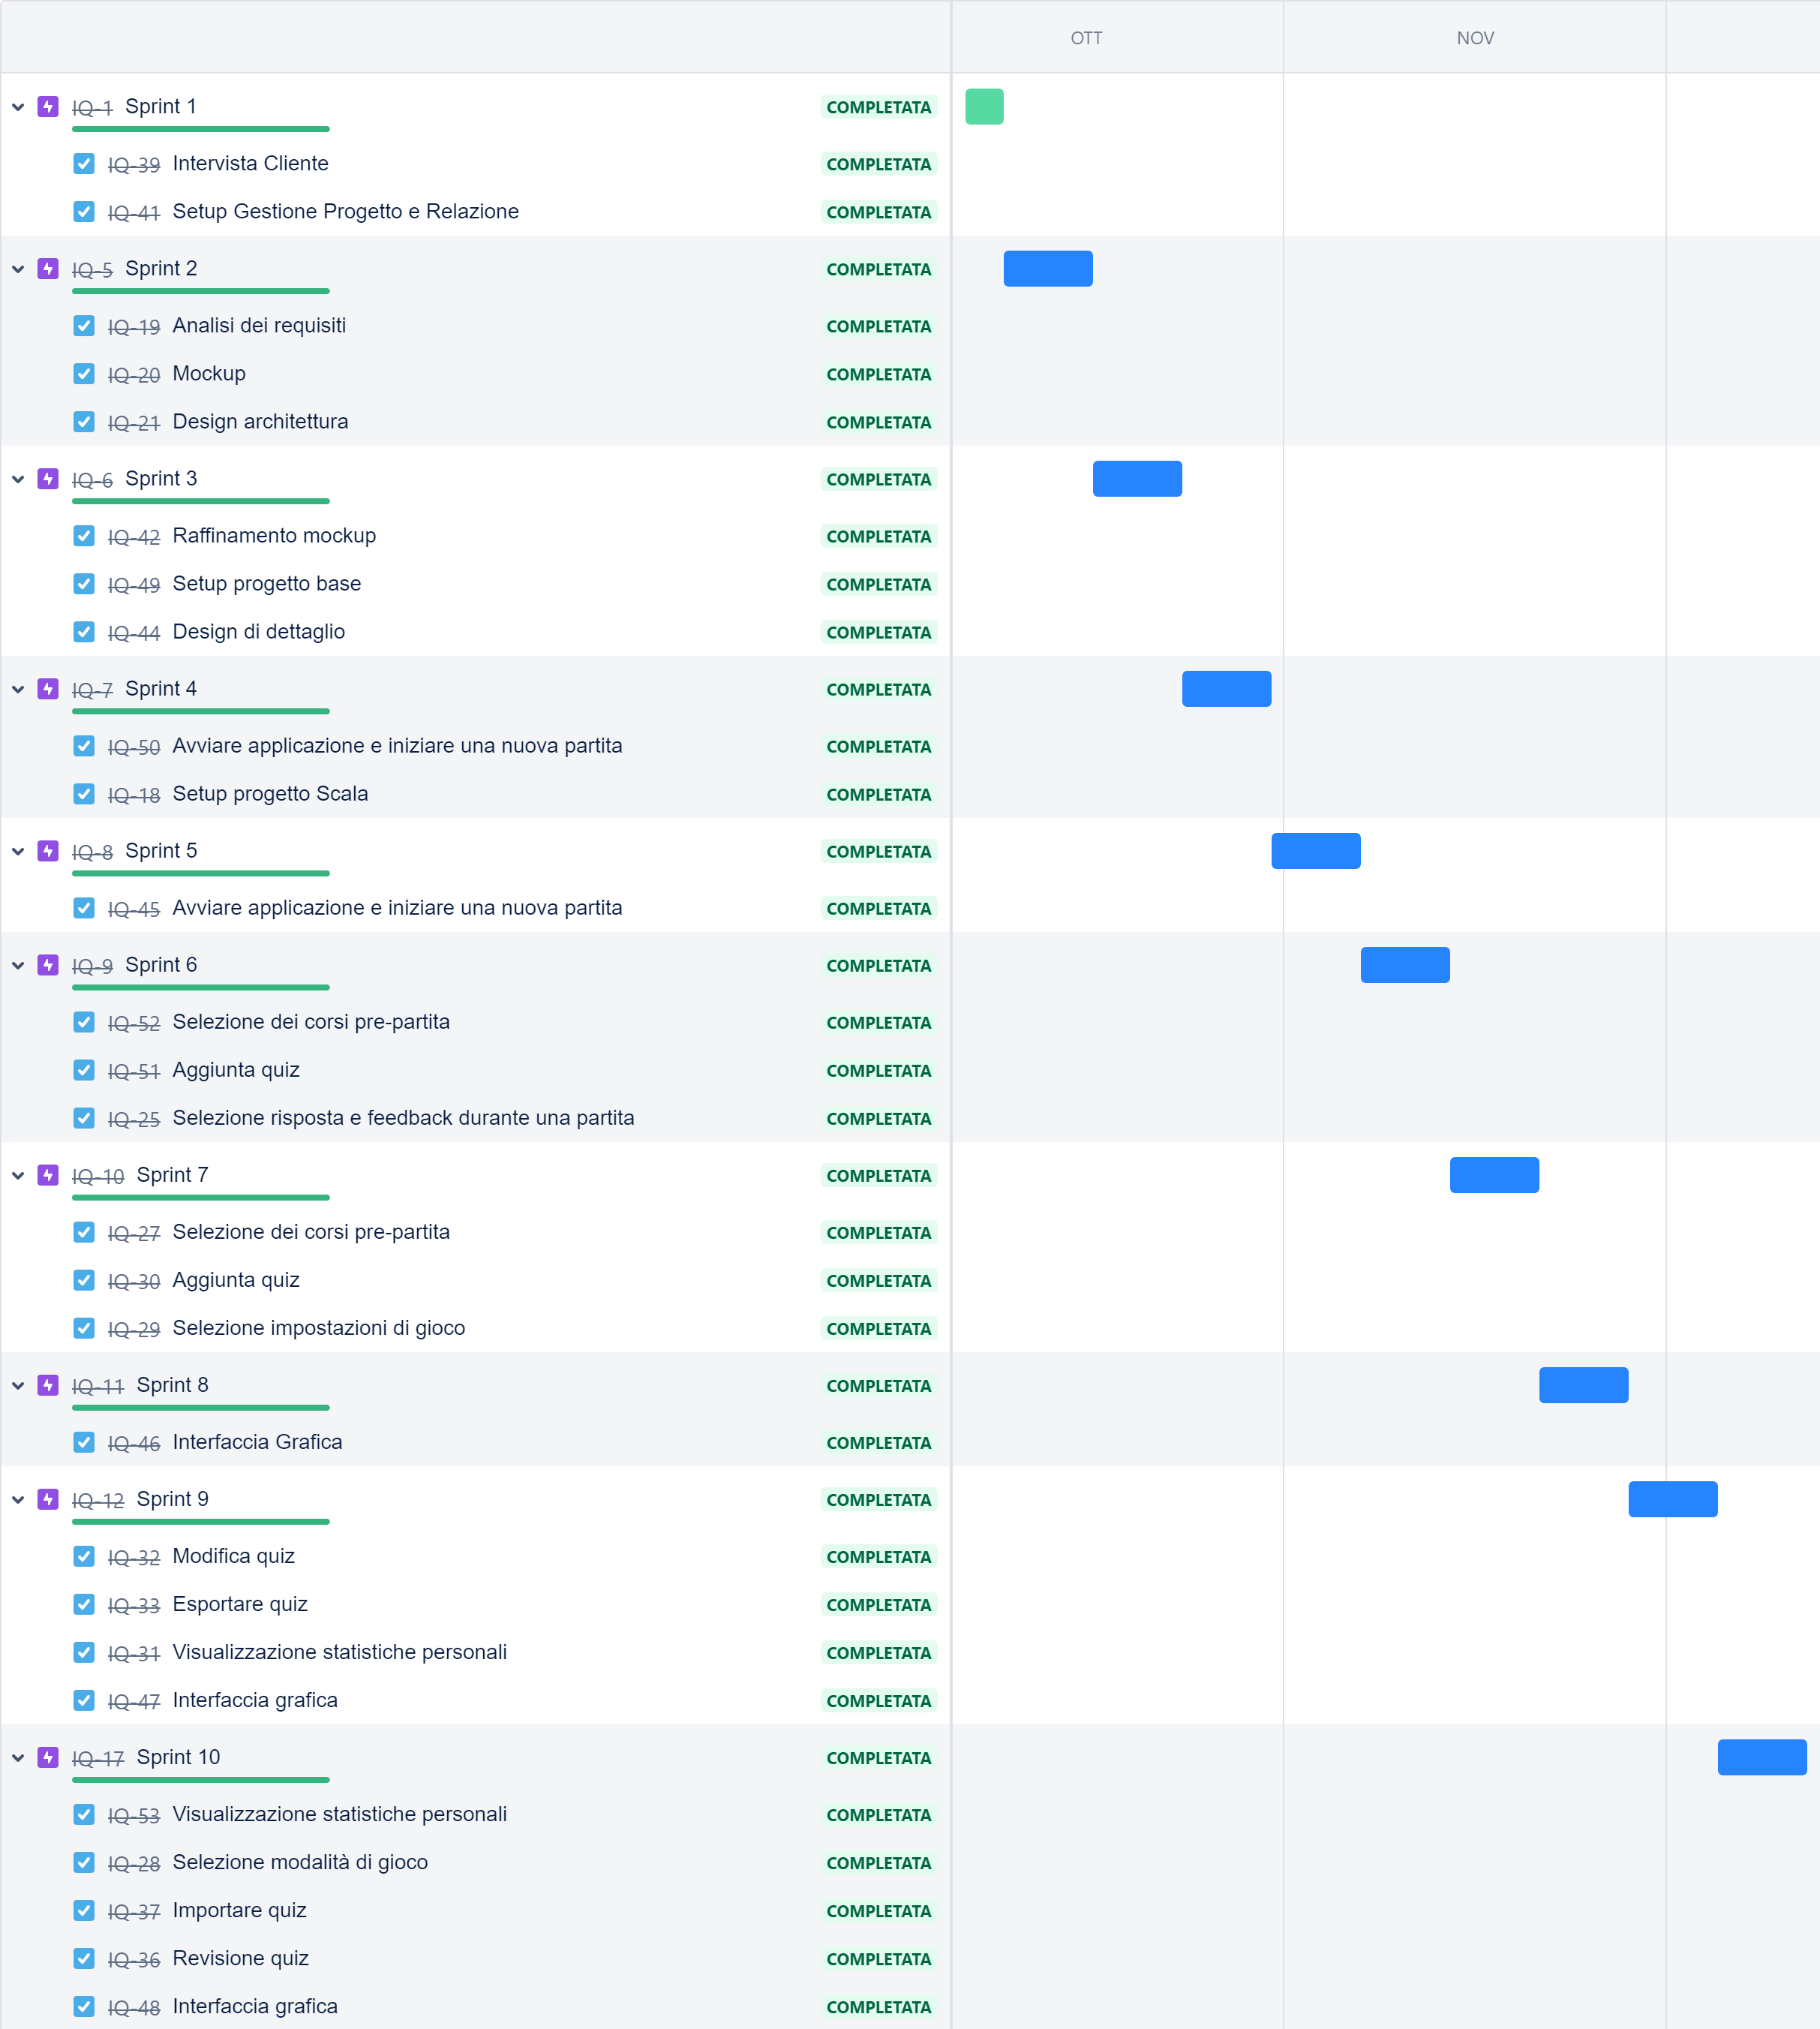
\includegraphics[width=\textwidth]{Images/Jira_final.png}
            \caption{Diagramma di Gantt aggiornato alla fine del progetto}
            \label{fig:jira-final}
        \end{figure}